\section{Introduction}
\label{sec:introduction}
The best way we know of describing the semantics of parametric
polymorphism is \emph{relational parametricity}, whose central result
is Reynolds' abstraction theorem~\cite{reynolds83types}. Its striking
consequences include the well-known ``free theorems'' for polymorphic
types~\cite{wadler89theorems}, non-inhabitation results, and precise
correspondences between System F encodings and algebraic
datatypes~\cite{PittsAM:parpoe}, abstract data types, and, most
recently, higher-order encodings of binder
syntax~\cite{syntaxforfree}.

Relational parametricity is in essence a principle of
\emph{invariance}: the behaviour of polymorphic code is invariant
under changes of data representation. Invariance results also abound in
mathematics and physics. The area of a triangle is invariant with
respect to isometries of the Euclidean plane; the determinant of a
matrix is invariant under changes of basis; and Newton's laws are the
same in all inertial frames. Typically, transformations in mathematics
and physics have interesting structure; for example, translations in
the Euclidean plane form an abelian group.

%Types express properties of programs. The statement $\mathit{b}:
%\tyBool$ tells us that $\mathit{b}$ has value $\mathtt{true}$ or
%$\mathtt{false}$; the statement
%$\mathit{pos}:\tyReal\tyProduct\tyReal$ says that $\mathit{pos}$ is a
%pair whose components are real numbers. More interestingly, the
%statement $\mathit{f} : \forall
%X. \tyPrim{list}X\tyArr\tyPrim{list}X$ tells us that if we apply
%$\mathit{f}$ to a list whose elements satisfy some property $\psi$,
%then the result is a list whose elements also satisfy $\psi$.

%Unary predicates only go so far, and for polymorphic types
%particularly do not express everything that follows from possessing
%that type.  Imagine a function $\mathit{oddRev}$ that reverses any
%list whose first element is an odd number, otherwise behaving as the
%identity. It certainly preserves properties of the elements -- but
%truly parametric polymorphism should tell us more.

%To obtain stronger properties we must \emph{relate} multiple
%executions of the same code. The statement $\mathit{f}:\forall
%X. \tyPrim{list}X\tyArr\tyPrim{list}X$ then says that any change in
%representation of the list elements supplied to $\mathit{f}$ is
%reflected in the elements in the result.  Formally, for any function
%$g$, we have $\mathit{f}(\mathrm{map}\:\mathit{g}\:\mathit{x}) =
%\mathrm{map}\:\mathit{g}\:(\mathit{f}\:\mathit{x})$.  This is the
%essence of \emph{relational parametricity} as formulated by
%Reynolds~\cite{reynolds83types}. Its consequences are striking.  It
%immediately tells us that $\mathit{oddRev}$ cannot be given a
%polymorphic type: simply consider the change-of-representation given
%by $\lambda x. x+1$.  But more profoundly it can be used to prove
%blah blah (initial algebras, term reps, non-inhabitation, etc.).

In previous work the third author studied relational parametricity for
types parameterized by units-of-measure, whose invariance 
properties relate to changes of units, or \emph{scaling}~\cite{kennedy97relational}. 
In this paper we investigate the general case of types indexed by attributes
with algebraic structure. For example, in computational geometry, points in
the plane can be indexed by a coordinate frame; in information-flow
security, computations are indexed by principals; in differential privacy, types
can be indexed by `distance'. Types that are
polymorphic over such indices induce invariance properties and
abstraction barriers beyond those introduced by their unindexed
versions, as we now illustrate.

\paragraph{Invariance}
A function $\mathit{areaTri}$ that computes the area of a triangle
can be assigned the type:
$\tyPrimNm{vec}\times\tyPrimNm{vec}\times\tyPrimNm{vec}\tyArr\tyReal$.
But we can also assign it the following more expressive polymorphic
type:
\[
\mathrm{areaTri} : \forall t\mathord:\SynTransl{2}.
  \tyPrim{vec}{t} \times \tyPrim{vec}{t} \times \tyPrim{vec}{t} \to \tyReal \\
\]
This type expresses the fact that if each of the arguments to $\mathrm{areaTri}$
is translated by the same vector, then the result remains the same,
that is, it is \emph{invariant} under translation. Formally, for any 
vector $\vec t$,
\[
\mathrm{areaTri}\;(\vec{t} + \vec{v_1}, \vec{t} + \vec{v_2}, \vec{t} + \vec{v_3}) = 
\mathrm{areaTri}\;(\vec{v_1}, \vec{v_2}, \vec{v_3})
\]

Transformations typically \emph{compose} in various
ways, and the compositions satisfy algebraic laws. For example, 
we can assign a function that computes the area of a circle given its
radius the following polymorphic type:
\[
\mathrm{areaCircle} : \forall s\mathord:\SynGL{1}.\tyPrim{real}{s}\to
\tyPrim{real}{s\cdot s}
\]
This captures the fact that the area of a circle varies as the square
of its radius, i.e., $\mathrm{areaCircle}(k r) = k^2\cdot
\mathrm{areaCircle}(r)$ for any $k\neq 0$ (i.e., any $k$ in the
one-dimensional general linear group $\GL{1}$).  Here, $s$ 
can be interpreted as the \emph{units of measure} of the argument to
$\mathrm{areaCircle}$, and `$\cdot$' composes units using the
product. We can also add an inverse operation and identity unit of
measure $1$, and then impose the algebraic laws of abelian
groups. This permits identification of, for example,
$\tyPrim{real}{s\cdot s^{-1}}$ with the type
$\tyPrim{real}{1}$ of dimensionless constants.

\paragraph{Abstraction}
In his original paper on parametricity, Reynolds asserted that
\emph{type structure is a syntactic discipline for enforcing levels of
  abstraction}.  We see something analogous here: if all primitive
operations are given types that reflect their behaviour under
translation, then there is no way to `break' this property. For
example, there is no way that $\mathrm{areaTri}$ can depend on the
actual coordinates of its inputs. Furthermore, the distinction between
points and vectors that is often enforced through abstract data
types~\cite{CGAL} is captured here by indices instead. For example,
the operation that takes two points and computes their vector
difference can be assigned the type
$\forall t\mathord:\SynTransl{2}.\tyPrim{vec}t\times\tyPrim{vec}t\to\tyPrim{vec}0$,
reflecting the invariance of the result (a pure vector) under
translations of the point arguments. As a result through types alone
we can, in essence, derive so-called \emph{coordinate-free}
geometry~\cite{CFGADT}.

The invariance properties discussed above can be seen as ``free
theorems''~\cite{wadler89theorems}, but the abstraction afforded by
polymorphic indexed types can also induce interesting type
\emph{isomorphisms}.  The type of $\mathrm{areaCircle}$ above is in
fact isomorphic to $\tyPrim{real}{1}$. A moment's thought reveals why:
what possible unary functions can be constructed whose outputs scale
as the square of the scaling of their inputs?  Answer: just those
functions of the form~$\lambda x. k x^2$ for some constant~$k$.  In
this case, of course, we expect that~$k = \pi$.

\paragraph{Relational parametricity}
To derive such invariance and abstraction properties of types, we
adopt the techniques of relational parametricity. Over an underlying
index-erasure semantics we construct binary relations parameterised by
an environment $\rho$ that describes how values of primitive type are
related according to their indices.  For example, values $v$ and $w$
of type $\tyPrim{real}\alpha$ are related when $v$ ``scales to'' $w$
according to an interpretation of $\alpha$ (i.e., $w=\rho(\alpha)\cdot
v$).  Values of polymorphic type are related exactly when they are
related for all possible interpretations of the quantified
variable. For example, values $v$ and $w$ of type
$\forall t\mathord:\SynTransl{2}.\tyPrim{vec} t\to
\tyPrim{vec} t$ are related when they are related at type
$\tyPrim{vec} t\to\tyPrim{vec}t$ for all translations
$\vec t\in\Transl{2}$ associated with $t$.

\vspace*{0.1in}

As it happens, the above examples can all be expressed using unary
functions rather than binary relations: we can write functions that
scale, or translate, one value to another according to their type,
even for higher-order function types. Moreover, the interpretation of
indices can be built up compositionally, by recursion over the
syntactic structure. For example, we have $\rho(\alpha\cdot\beta) =
\rho(\alpha)\cdot\rho(\beta)$ where product of units-of-measure is
interpreted by product of scale factors. For more sophisticated
applications, however, we need the fully generality of binary
relations. As is the case with type polymorphism, it
provides the appropriate meaning for nested quantifiers in types such
as
$(\forall s\mathord:\SynGL{1}.\tyPrim{real} s\to\tyPrim{real} s)\to\tyBool$.
More interestingly, particular applications sometimes require
relations that are not built compositionally---we can, for instance,
use such relations to prove that there are no non-trivial programs of
type
$\forall s\mathord:\SynGL{1}.\tyPrim{real}{s\cdot s}\to\tyPrim{real}s$.
Finally, there are interesting applications in which even the basic
relations are not functional. In a type system in which the index in
$\tyPrim{real}s$ is interpreted not as a unit of measure, but as
a measure of \emph{closeness}, two values $x$ and $y$ of this type are
related if $|x-y| < \rho(s)$ for a positive real number
$\rho(s)$.  Rather beautifully, the standard notion of uniform
continuity can then be expressed as %a type:
%\begin{displaymath}
 $ \forall \epsilon \mathord: \mathsf{R}^{>0}.\ \exists \delta\mathord: \mathsf{R}^{>0}.\ \tyPrim{real}{\delta} \to \tyPrim{real}{\epsilon}$.
%\end{displaymath}


% Possible angles of attack:
% \begin{itemize}
% \item Parametric polymorphic types allow us to prevent
%   over-specification of the behaviour of programs. For instance, the
%   type $\forall \alpha. [\alpha] \to [\alpha]$ is a generalisation of
%   the types $[\mathsf{int}] \to [\mathsf{int}]$ and $[\mathsf{char}]
%   \to [\mathsf{char}]$. Either of the latter two types over-specify
%   the behaviour of the function.
% \item There are other cases of programs that are over-specified. The
%   leading example we just below is of geometric programs that
%   manipulate coordinate data. Often, programs that manipulate
%   coordinate data are insensitive to geometric transformations. For
%   example, a program that computes the area of a triangle described by
%   three points is insensitive to translations or rotations applied to
%   all three points.
% \item 
% \end{itemize}

% There are three main points to get across:
% \begin{enumerate}
% \item Why algebraically indexed types?
% \item Why relational parametricity?
% \item Why study them together?
% \end{enumerate}

\subsection{Contributions}
\label{sec:contributions}

\begin{figure}
  \centering
  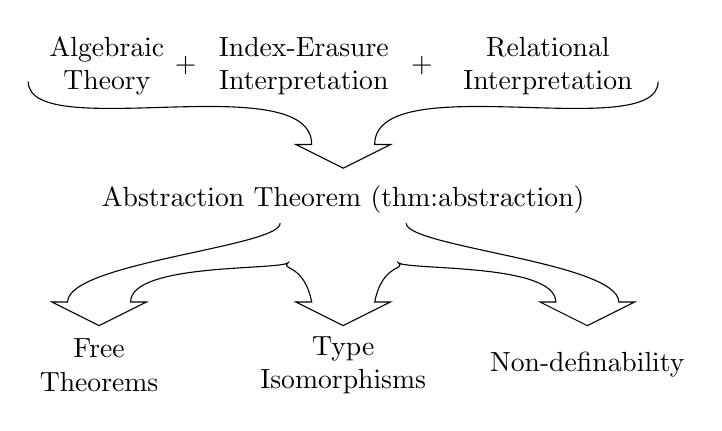
\begin{tikzpicture}
  \node at (-3,1) [rectangle,style={align=center}] {Algebraic \\ Theory};
  \node at (-2,1) {$+$};
  \node at (-0.5,1) [rectangle,style={align=center}] {Index-Erasure \\ Interpretation};
  \node at (1,1) {$+$};
  \node at (2.6,1) [rectangle,style={align=center}] {Relational \\ Interpretation};
  
  \draw plot (-4,0.8) .. controls (-4,0) and (-0.4,1) .. (-0.4,0)
             -- (-0.6,0) -- (0,-0.3) -- (0.6,0) --
             (0.4,0) .. controls (0.4,1) and (4,0) .. (4,0.8);

  \node at (0,-0.7) [rectangle,style={align=center}] {Abstraction Theorem (\thmref{thm:abstraction})};

  \draw plot (-0.8,-1) .. controls (-0.8,-1.3) and (-3.5,-1.5) .. (-3.5,-2)
             -- (-3.7,-2) -- (-3.1,-2.3) -- (-2.5,-2) -- 
             (-2.7,-2) .. controls (-2.7,-1.5) and (-0.8,-1.6) .. (-0.7,-1.5)
                       .. controls (-0.8,-1.6) and (-0.5,-1.5) ..
             (-0.4,-2) -- (-0.6,-2) -- (0,-2.3) -- (0.6,-2) --
             (0.4,-2) .. controls (0.5,-1.5) and (0.8,-1.6) .. (0.7,-1.5)
                      .. controls (0.8,-1.6) and (2.7,-1.5) ..
             (2.7,-2) -- (2.5,-2) -- (3.1,-2.3) -- (3.7,-2) -- (3.5,-2)
                      .. controls (3.5,-1.5) and (0.8,-1.3) .. (0.8,-1);

  \node at (-3.1,-2.8) [rectangle,style={align=center}] {Free \\ Theorems};
  \node at (0,-2.8) [rectangle,style={align=center}] {Type \\ Isomorphisms};
  \node at (3.1,-2.8) [rectangle,style={align=center}] {Non-definability};
\end{tikzpicture}
  \caption{Summary of the Paper}
  \label{fig:summary}
\end{figure}

This paper makes the following specific contributions:
\begin{itemize}
\item 
We present a collection of compelling examples of algebraically
indexed types, including a novel type system for geometry, a
refined type system for information flow based on logic, and a simple
type system with distance-indexed types.
\item 
We formulate a type system that can either be used as a programming
language in its own right, or as the target of type-based
analyses. The type system consists of the usual type constructors
together with a collection of indexed primitive types, universal and
existential quantification over the indices, and a multi-sorted
equational theory for indices.
\item
We describe a relational semantics for the type system and prove an
analogue of Reynolds' abstraction theorem. We give precise conditions
on sets of relation environments under which our abstraction theorem
holds.
\item
For each of our main examples we deduce free theorems that are
consequences of our abstraction theorem, prove non-definability
results, and derive interesting type isomorphisms.
\end{itemize}
We have fully formalised our framework and most examples in Coq,
using strongly-typed term representations
throughout~\cite{TypedSyntax}. The formalisation is available from
\\{\small \url{https://github.com/bobatkey/algebraically-indexed-types}}



%%% Local Variables:
%%% TeX-master: "paper"
%%% End:
